\documentclass[conference]{IEEEtran}
\IEEEoverridecommandlockouts
% The preceding line is only needed to identify funding in the first footnote. If that is unneeded, please comment it out.
\usepackage{float}
\usepackage{cite}
\usepackage{amsmath,amssymb,amsfonts}
% \usepackage{algorithmic}
\usepackage{graphicx}
\usepackage{textcomp}
\def\BibTeX{{\rm B\kern-.05em{\sc i\kern-.025em b}\kern-.08em
    T\kern-.1667em\lower.7ex\hbox{E}\kern-.125emX}}
\begin{document}

\title{Image Steganography\\
}

\author{\IEEEauthorblockN{Saketh Katari}
\IEEEauthorblockA{\textit{Computer Science Department} \\
\textit{IIIT-Delhi}\\
Delhi, India \\
katari15045@iiitd.ac.in}
}

\maketitle

\begin{abstract}
This document explains a new strategy to transfer confidential data by combining steganography with cryptography.
LSB steganography is further improved by randomly storing confidential data in an image which makes it difficult to retrieve.
Considering human visual system, it is difficult for the user to detect the changes in stego image. \\
\end{abstract} 

\begin{IEEEkeywords}
steganography, LSB, image, cryptography, random
\end{IEEEkeywords}

\section{Introduction}
Confidential data is everywhere and it is necessary to transfer it securely over internet.
Cryptography comes into picture when the data is with you but nothing is made out of it, as it is a cipher, making no sense.
Steganography hides confidential data within some other data (say image) and makes it difficult to even detect that there is a secret here.
Cryptography combined with steganography provides a 2 layer protection - detecting the confidential data (steganography) and making sense out of it (Cryptography).\\

Images are used (among audio, video, text etc) as a medium to store the confidential data.
Any data such as text, image, audio etc can be embedded in an image and is tranferred to the destination.
If an attacker sees this image, it would be difficult to detect that there is some hidden data in it, as it looks lika a normal image.\\

\section{Related work}
Most of the traditional LSB steganography techniques store the confidential data in the LSBs (Least Significant Bit) of every pixel without any randomization, as shown below
\cite{b1}. 
\\ \\
\centerline{ Confidential data }
\centerline{ 100110011 }
\leavevmode \\ \\ \\
\centerline{ Pixels before embedding confidential data }
\leavevmode \\ \\
\centerline{ R \\ G \\ B }
\centerline{ 10010110 \\ 01101111 \\ 01101011 }
\centerline{ 01011100 \\ 11000110 \\ 01000011 }
\centerline{ 10111111 \\ 11100110 \\ 00101110 }
\leavevmode \\ \\ \\
\centerline{ Pixels after embedding confidential data }
\leavevmode \\ \\
\centerline{ R \\ G \\ B }
\centerline{ 1001011\textbf{1} \\ 0110111\textbf{0} \\ 0110101\textbf{0} }
\centerline{ 0101110\textbf{1} \\ 1100011\textbf{1} \\ 0100001\textbf{0} }
\centerline{ 1011111\textbf{0} \\ 1110011\textbf{1} \\ 0010111\textbf{1} }
\leavevmode \\ \\

During this process, the LSBs of some pixels are replaced, which modifies the image.
LSB has less effect (changes by 1) on the overall value; hence it is modified instead of MSB.\\ 

However, this is not secure because, an attacker might just access the LSBs of every pixel and retrieve the confidential data. 
Instead, some randomization is necessary while embedding data so that, when an attacker tries to retrieve data, it is difficult to produce the same pattern that was randomly generated.\\

It is necessary to transfer the random pattern to the destination to retrieve data that is embedded. \\


The performance of a method or an algorithm is evaluated on the basis of the change in the image before and after embedding data in it.
An algorithm is considered better if it produces minimal change in the image after embedding data in it.\\

\section{Proposed model}
This model adds cryptography and randomization to the traditional LSB steganographic techniques.
\\
\subsection{Notation}
Cover\_image - The image (before embedding) that is supposed to carry the confidential data in it. \\

Stego\_image - The image (after embedding) that contains confidential data in it. \\

location\_data - Meta data (Data about confidential\_data) that identifies the location of confidential\_data within a stego\_image. \\

Component\_of\_a\_pixel - The Red, Green and the Blue components (RGB). \\

LSB - Least Significant Bit of a binary number. \\

pr\_key\_src - Sender's private key \\

pr\_key\_dest - Receiver's private key \\

pub\_key\_src - Sender's public key \\

pub\_key\_dest - Receiver's public key \\
\subsection{Overview}
\leavevmode \\ \\
\centerline{Cover Image + Confidential data + Location data}
\leavevmode \\ \\
\centerline{$\downarrow$}
\leavevmode \\ \\
\centerline{ Stego image }
\leavevmode \\ \\
\centerline{$\downarrow$}
\leavevmode \\ \\
\centerline{ Encrypted Stego image }
\leavevmode \\ \\
\centerline{ Location Data \\ {$\rightarrow$} \\ Encrypted location data}
\leavevmode \\ \\
\centerline{---------------------------} 
\leavevmode \\ \\
\centerline{ Encrypted stego image + Encrypted location data }
\leavevmode \\ \\
\centerline{$\downarrow$}
\centerline{Internet}
\leavevmode \\ \\
\centerline{$\downarrow$}
\centerline{Destination}
\leavevmode \\ \\
\centerline{---------------------------} 
\leavevmode \\ \\
\centerline{ Encrypted data }
\leavevmode \\ \\
\centerline{$\downarrow$}
\leavevmode \\ \\
\centerline{ Decrypted stego image + decrypted location data }
\leavevmode \\ \\
\centerline{$\downarrow$}
\leavevmode \\ \\
\centerline{ Confidential data }
\leavevmode \\ \\

\subsection{Pre-processing}
A random location\_data is generated with necessary length (typically, equal to the size of confidential\_data). Let it be 'abc'.
This is converted to 8-bit ASCII values '97, 98, 99'.
Finally, it is converted to a binary string '01100001, 01100010, 01100011'.\\

Similarly, another binary string is produced for the confidential\_data.\\

\subsection{Embedding}

\begin{figure}[H]
  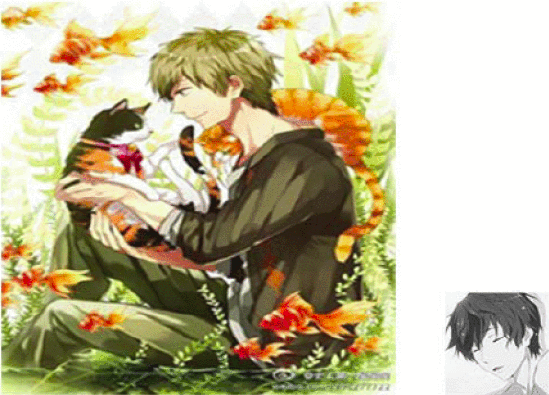
\includegraphics[width=\linewidth]{cover_image_cum_confidential_data.png}
  \caption{Left - Cover\_image, right - confidential\_data\_image \cite{b2}.}
\end{figure}

Grayscale image (Black and white) in Fig.1 is to be embedded in the color image to it's left.\\

Each bit is taken from the confidential\_data and from the location\_data;
let them be c\_bit and l\_bit respectively.
c\_bit is embedded in one of the components of a pixel which is determined by l\_bit.\\

It is observerd that the human eye is most sensitive to the green component of the light \cite{b2}.
So, LSB of the green component is not replaced.\\

A pixel is chosen in lexicographical order (row\_number, column\_number in lexicographical order).
For a given l\_bit and c\_bit, l\_bit is XORed with LSB of green component.
If it gives 0, LSB of blue is replaced with c\_bit, else, LSB of red is replaced with c\_bit \cite{b2}.\\

\begin{figure}[H]
  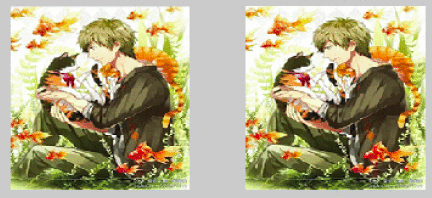
\includegraphics[width=\linewidth]{cover_image_vs_stego_image.png}
  \caption{Left - Cover\_image, right - stego\_image \cite{b2}.}
\end{figure}

As you can see in Fig.2, it is difficult to distinguish between the left (before embedding confidential\_data) and right images (after embedding confidential\_data)

\subsection{Encryption}
Stego\_image is first encrypted by the pr\_key\_src and then encrypted with the pub\_key\_dest.
Encrypting with pr\_key\_src is referred as a digital signature.
pub\_key\_dest makes sure that only destination can decrypt it with it's private key \cite{b2}.\\

\centerline{ pub\_key\_dest ( pr\_key\_src ( data ) ) }
\leavevmode \\
Similarly, location\_data is encrypted.\\

Now, stego\_image along with location\_data is transferred to destination.

\subsection{Decrpytion}
Stego\_image is first decrypted using the pr\_key\_dest and then with the pub\_key\_src.
Now, the receiver has the decrypted stego\_image .\\

\centerline{ pub\_key\_src ( pr\_key\_dest ( data ) ) }
\leavevmode \\

Similarly, decrypt the location\_data. \\
\subsection{Extracting embedded data}
A pixel is chosen in lexicographical order (row\_number, column\_number in lexicographical order).
For each bit l\_bit in location\_data, XOR l\_bit with the LSB of the green component.
If it's 0, append the LSB of blue to the confidential\_data, else, append the LSB of red to the confidential\_data.\\
\\ \\
\centerline{l\_bit - 1}
\leavevmode \\ \\
\centerline{Pixel - }
\centerline{R(10010111)}
\centerline{G(0110111\textbf{0})}
\centerline{B(01101010)}
\leavevmode \\ \\
\centerline{c\_bit = LSB\_of\_Green \textbf{XOR} l\_bit}
\centerline{ = 0 \textbf{XOR} 1 = 1 i.e LSB of red component = 1 }
\leavevmode \\ \\

Similarly, construct the whole confidential\_data which results in a binary string.
Convert this binary string to 8-bit ASCII values and finally to ASCII characters.\\
\subsection{PSNR (Peak Signal to Noise Ratio)}
As name indicates, it is the ratio of signal to noise.
Higher the PSNR lesser the noise in an image.\\

PSNR of traditional LSB based steganography techniques is around 53 db \cite{b1}.
This method gives a PSNR of around 56 db, better than traditional PSNR.\\  
\subsection{Security}
It has two layers of security - steganography and cryptography.\\

It's difficult to detect confidential\_data that is embedded in an image.
If an attacker somehow gets encrypted data, it's difficult to decrypt it.\\
\section{Conclusion}
Traditional LSB steganography technique has been improved in three ways -\\ \\
1. Two way security with cryptography.\\
2. Making it difficult for an attacker to predict the random pattern that is used to embed confidential\_data in a cover\_image.\\
3. PSNR is increased from 53 db to 56 db.\\
\section*{Acknowledgment}
I would like to thank 'Technical Communication [COM 301A]' staff and IIIT-Delhi (Indraprastha Institute of Information Technology).\\

\begin{thebibliography}{00}
\bibitem{b1} S. M. Masud Karim, Md. Saifur Rahman, Md. Ismail Hossain, "A new approach for LSB based image steganography using secret key".  Computer and Information Technology (ICCIT), 2011 14th International Conference, 22-24 Dec. 2011, Dhaka, Bangladesh.\\
\bibitem{b2} Xinyi Zhou, Wei Gong, WenLong Fu, LianJing Jin, "An improved method for LSB based color image steganography combined with cryptography". Computer and Information Science (ICIS), 2016 IEEE/ACIS 15th International Conference, 26-29 June 2016, Okayama, Japan.\\
\end{thebibliography}

\end{document}
